
% ----------------------------------------------------
% Institute of Medical Informatics
% University of Luebeck
%
% Version 0.4
%
% ----------------------------------------------------

\documentclass[
%a4paper,
12pt,
headsepline,
bibliography=totoc,
twoside=semi,
fleqn
]{scrartcl}

\usepackage{pgf}
\usepackage{ucs}
\usepackage[latin1]{inputenc}
%\usepackage[pdftex]{graphicx}
\graphicspath{{./images/}}
\usepackage{color}
%\usepackage{german}
\usepackage{subfigure}
\usepackage{booktabs}

%% LAYOUT:

\renewcommand{\descfont}{\bfseries}
\renewcommand{\sectfont}{\bfseries}

\addtolength{\topmargin}{-1.5cm}
\addtolength{\textheight}{1.5cm}

\setkomafont{captionlabel}{\bfseries\footnotesize}
\setkomafont{caption}{\footnotesize}
\renewcommand{\headfont}{\bfseries}
\renewcommand{\figurename}{Fig.}
\renewcommand{\tablename}{Table}

\renewcommand*{\titlepagestyle}{empty}

\usepackage[automark]{scrlayer-scrpage}
\pagestyle{scrheadings}
\clearscrheadfoot
\rehead{\headmark} 
\lehead{\pagemark} 
\lohead{\headmark} 
\rohead{\pagemark}

\definecolor{Ocean}{cmyk}{1,0,0.2,0.78}
\definecolor{Grey}{cmyk}{0,0,0,0.6}

\usepackage{natbib}
\bibpunct{[}{]}{;}{a}{}{,}

\begin{document}

%==================================================
% TITLE PAGE
% -------------------------------------------------

\setlength{\headheight}{0pt}

\titlehead{
  \flushleft{
\includegraphics[width=0.7\textwidth]{Logo_Inst_MedInformatik_En_P309}}\\[-3.5ex]
  \centering
}

\subject{
\large{
  \vspace{0ex}
  \textnormal{Seminar}\\[1ex] 
  Medical Image Computing and e-Health\\[1ex]
  \textnormal{WS 20??/20??}\\[8ex]
}}

\title{
  \huge{\textcolor{Ocean}{Title}}\\[5ex]
}

\author{
  \large{\textbf{Name Student}}\\
  \large{Matr.-Nr.: XXXXXXX, Field of Study}\\[5ex]
  \large{Supervisor:}\\
  \large{Name Supervisor}\\[8ex]
}

\date{
  \large{L¸beck, \today}
  \pgfdeclareimage{university-slogan}{./images/Slogan_Uni_Luebeck_CMYK}
  \begin{pgfpicture}{0cm}{4cm}{14cm}{1.0cm}
    \pgfputat{\pgfpoint{10cm}{0cm}}{\pgfbox[left,bottom]{\pgfuseimage{university-slogan}}}
    \color {white}
%    \pgfputat{\pgfpoint{12.3cm}{0.4cm}}{\pgfbox[right,center]{  \insertshorttitle}}	
  \end{pgfpicture}
}

\maketitle

\setcounter{page}{1}
\setlength{\headheight}{58pt}

%==================================================

\tableofcontents
%\newpage

%==================================================
% TEXT
% -------------------------------------------------

\section{Introduction\label{sec:sec1}}

This is an IMI TeX template for seminar papers (here: BSc seminar ``Medizinische Informatik / eHealth, AI and Medical Image Computing - CS3703''). Contributors, topics of the presentations, important dates, and supervisors are summarized in Table~\ref{tab:table1}. Further information can also be found in Moodle (Fig.~\ref{fig:subfigureExample}).

%--------------------------------------------------

\section{Seminar-specific Details\label{sec:sec2}}


\subsection{Dates\label{sec:sec2-1}}

Important dates (in addition to Table~\ref{tab:table1}):

\begin{itemize}
  \item Contact your supervisior before the \textbf{2020-10-30} to discuss the paper to be presented.
  \item Deadline for the final and approved version of the presentation: \textbf{2020-12-18}
  \item Abstract over 300 to 500 word due on \textbf{2020-12-18}
  \item Deadline for seminar papers: \textbf{2021-02-28}. We highly recommend to send the paper to your supervisor \underline{well in advance} (approx. 2 weeks before deadline) to allow him/her to suggest improvements etc..
  \item Last date for the resubmission of the articles approved by the supervisor: \textbf{2021-03-31}
\end{itemize}

\noindent Presence at all presentations is of course mandatory (if possible; otherwise please send an email to your supervisor).


\subsection{Guidelines\label{sec:sec2-2}}

\subsubsection{Presentation}
 
Presentation time is approximately 30 min + discussion for Bachelor students. Please note that the contents should be presented in an easy-to-understand manner, i.e. all participants of the seminar should be able to follow your presentation! Powerpoint and LaTeX (Beamer) templates are provided on Moodle. Using other layouts and file formats is of course possible. To prevent technical issues (problems with video codecs etc.) we recommend that you bring your \underline{own notebook}.

\subsubsection{Paper} 

The seminar paper should roughly span 8-10 pages and be sent to the supervisor by email in pdf file format.


%--------------------------------------------------
% Example of a figure with subfigures
%--------------------------------------------------

\begin{figure}[p]
\centering
\subfigure[]{
  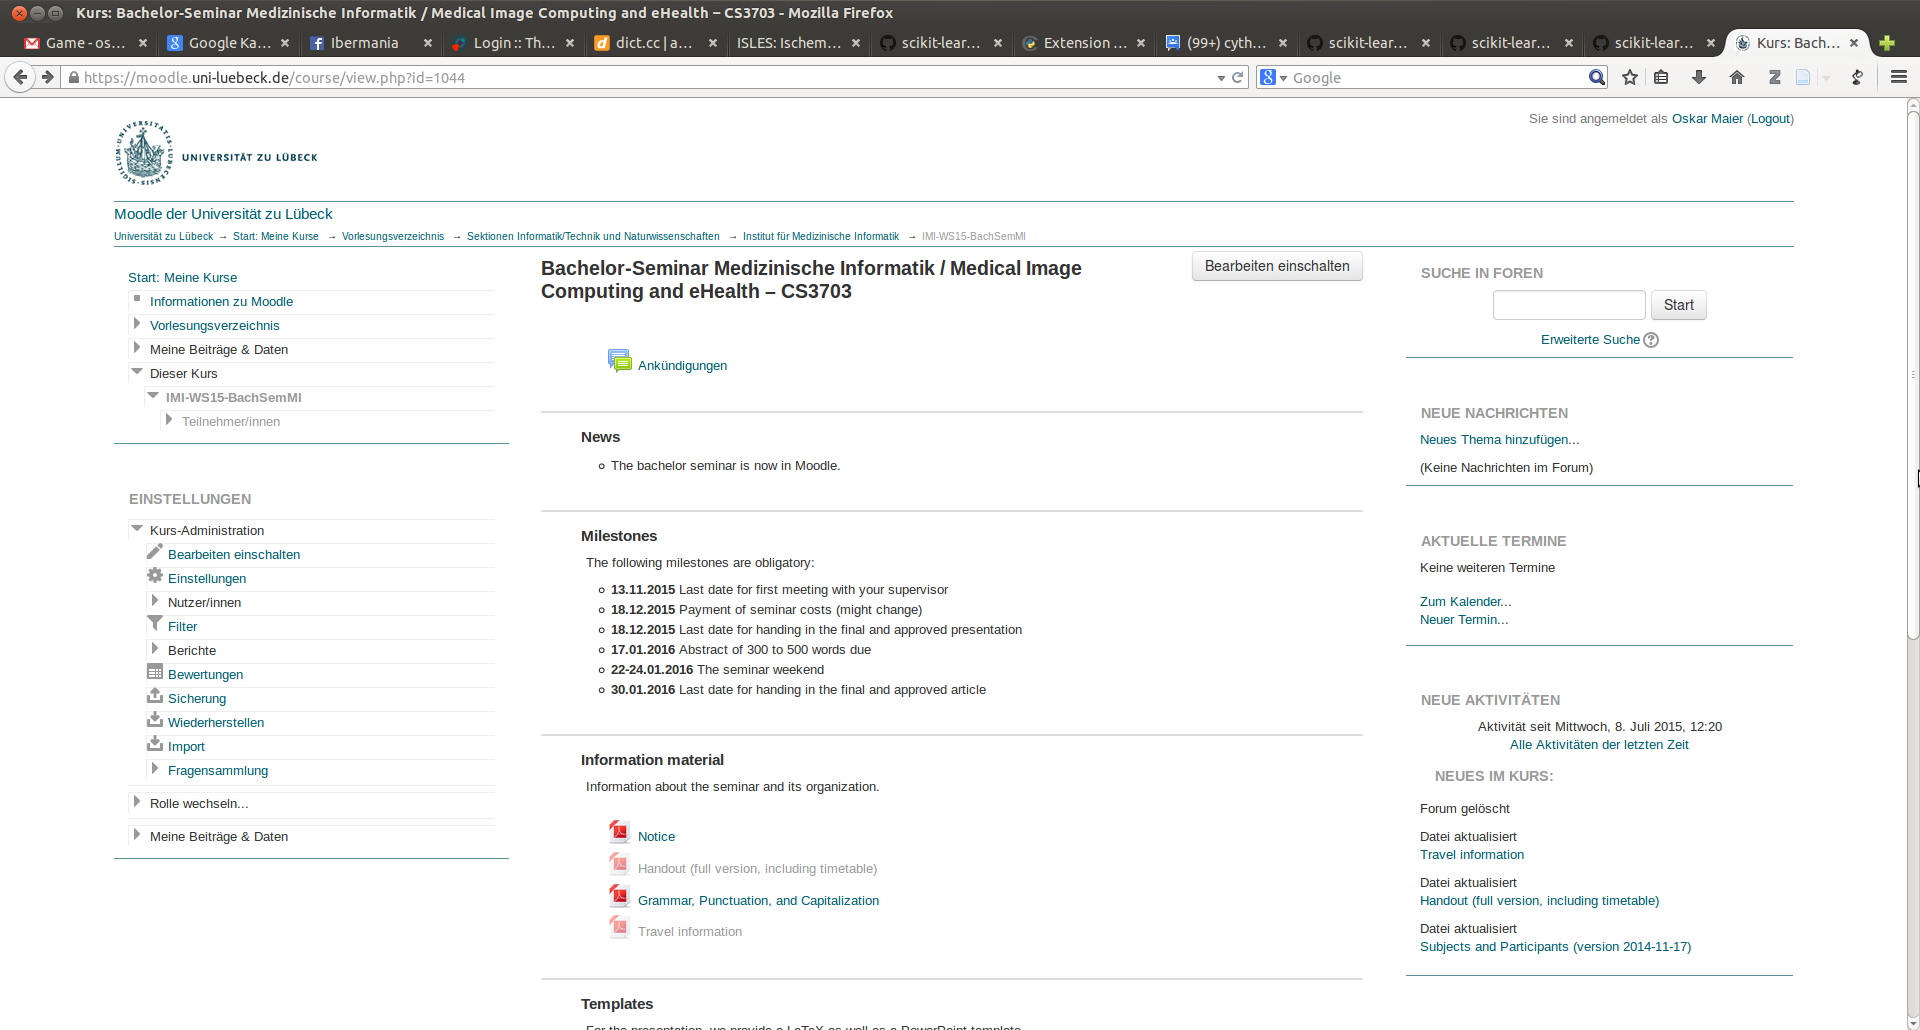
\includegraphics[width=\textwidth]{Moodle4}
  \label{fig:subfig1}
}
\subfigure[]{
  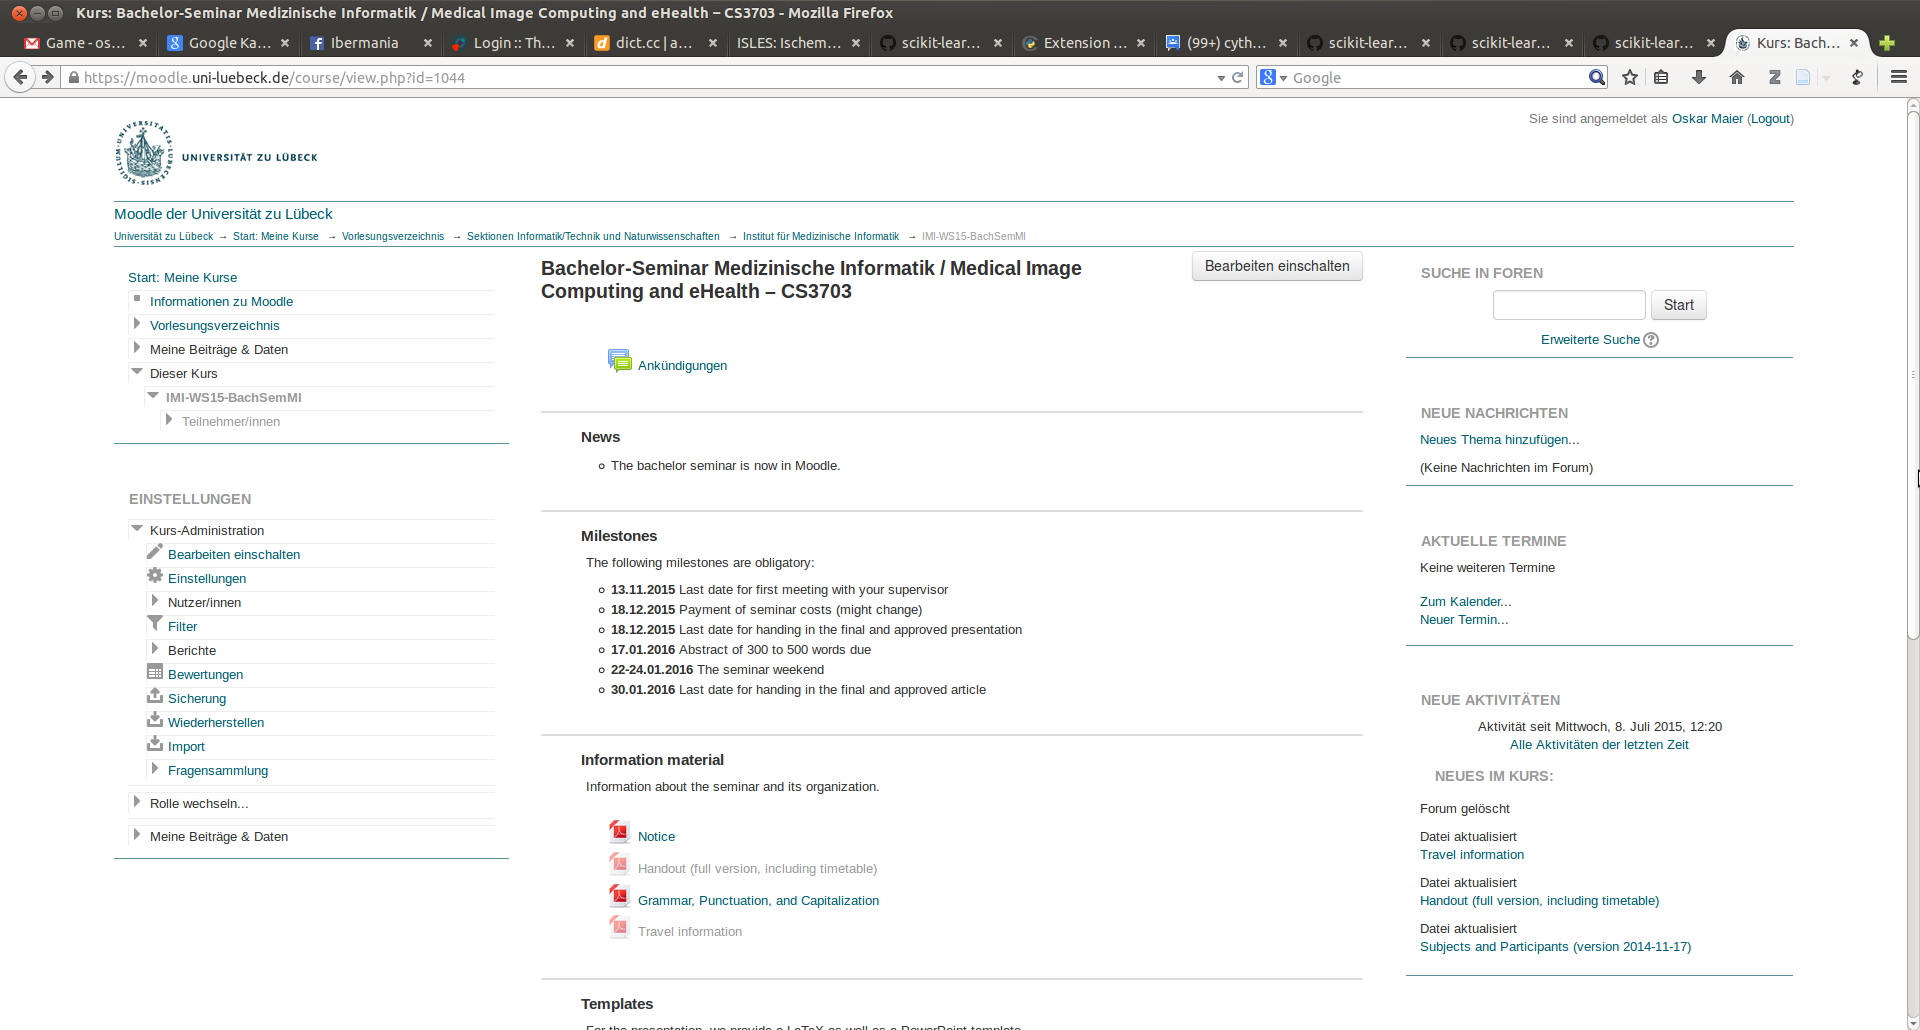
\includegraphics[width=\textwidth]{Moodle4}
  \label{fig:subfig2}
}
\caption{Two times (\subref{fig:subfig1} and \subref{fig:subfig2}) the Moodle page for this seminar.}
\label{fig:subfigureExample}
\end{figure}

%--------------------------------------------------
% Example of a table
%--------------------------------------------------


\begin{table}[t]
\footnotesize
\caption{\label{tab:table1} Topics of the presentations \textbf{two years ago}.}
\vspace{1ex}
\centering 
\begin{tabular}{p{2.5cm}p{8.7cm}p{2.8cm}}
\toprule
\textbf{Speaker} & \textbf{Topic [Literature]} & \textbf{Supervisor} \\
\midrule
J. Niemeijer & Hough transforms & M. Wilms \\
D. Labitzke & Optimal Surface Segmentation in Volumetric Images -- A Graph-Theoretic Approach (cf. \citep{Li_TPAMI_2006}) & M. Wilms \\
A. Bostelmann & Graph Cuts for image segmentation
 & O. Maier \\
D. Conrad & Texture descriptors and their application to medical images & O. Maier
 \\
E. Franke & Image Segmentation Using Deformable Models: Parametric Deformable
Models & J. Kr¸ger \\
N. Broecker & Image Segmentation Using Deformable Models:Geometric Deformable
Models & J. Kr¸ger \\
L. Pankert & Visualization in Medicine: Volume Rendering with ray-casting
 & J. Ehrhardt \\
T. Langer & Visualization in Medicine: Surface Rendering using the Marching Cubes
Algorithm & J. Ehrhardt \\
M. Caspe & Volumetric Ultrasound Stitching & D. Fortmeier \\
H. Tˆnnies & Surface-based Palpation Haptics & D. Fortmeier \\
\midrule
P. Kling & A Content Model for the ICD-11 Revision & J. Ingenerf \\
S. Heusel & MeSHy: Mining unanticipated PubMed information using frequencies of
occurrences and concurrences of MeSH terms & J. Ingenerf \\
K. Soika & What is bioinformatics? An introduction and overview & B. Andersen \\
M. Licht & How (not) to protect genomic data privacy in a distributed network: using trail
re-identification to evaluate and design anonymity protection systems & J. Ingenerf \\
J. Fleckner & Adverse events in medicine: Easy to count, complicated to understand, and
complex to prevent & A.-K. Kock \\
A. Wiegmann & An automated technique for identifying associations between medications,
laboratory results and problems & A.-K. Kock \\
J.-H. Mathes & Organization of Heterogeneous Scientific Data Using the EAV/CR
Representation & B. Andersen\\
F. Simon & Structured Reporting: Patient Care Enhancement or Productivity Nightmare? & A.-K. Kock\\
\bottomrule
\end{tabular}
\vspace{2ex}
\end{table}


%==================================================
\newpage
%\bibliographystyle{plain}
\bibliographystyle{elsarticle-harv}
\footnotesize\bibliography{bib}

\end{document}
